\documentclass{article}
\usepackage{geometry}
\usepackage{graphicx}
\usepackage{float}
\geometry{a4paper, margin=1in}

\title{\textbf{Design and Synthesis of a 32-bit RISC Processor}\\[0.5em]
\large CS39001: Computer Organization and Architecture Laboratory}
\author{Group 06: Harshit Jain (22CS10030), Sachish Singla (22CS30046)}
\date{22nd October 2024}


\begin{document}

\maketitle

\tableofcontents
\newpage

\section{ Instruction Format and Encoding}

\subsection{R-Type Instructions}
\begin{table}[H]
    \centering
    \begin{tabular}{|c|c|c|c|c|c|}
        \hline
        \textbf{opcode} & \textbf{rs} & \textbf{rt} & \textbf{rd} & \textbf{Don't Care} & \textbf{func} \\
        \hline
        6 bits & 5 bits & 5 bits & 5 bits & 6 bits & 5 bits \\
        \hline
    \end{tabular}
    \caption{R-type Instruction Format}
\end{table}

\begin{table}[H]
    \centering
    \begin{tabular}{|c|c|c|c|}
        \hline
        \textbf{Instruction} & \textbf{Usage} & \textbf{Opcode} & \textbf{Function} \\
        \hline
        ADD & ADD rd,rs,rt & 000000 & 00001 \\
        SUB & SUB rd,rs,rt & 000000 & 00010 \\
        AND & AND rd,rs,rt & 000000 & 00011 \\
        OR  & OR rd,rs,rt & 000000 & 00100 \\
        XOR & XOR rd,rs,rt & 000000 & 00101 \\
        NOR & NOR rd,rs,rt & 000000 & 00110 \\
        SL  & SL rd,rs,rt  & 000000 & 00111 \\
        SRL & SRL rd,rs,rt & 000000 & 01000 \\
        SRA & SRA rd,rs,rt & 000000 & 01001 \\
        SLT & SLT rd,rs,rt & 000000 & 01010 \\
        SGT & SGT rd,rs,rt & 000000 & 01011 \\
        NOT & NOT rd,rs & 000000 & 01100 \\
        INC & INC rd,rs & 000000 & 01101 \\
        DEC & DEC rd,rs & 000000 & 01110 \\
        HAM & HAM rd,rs & 000000 & 01111 \\
        MOVE & MOVE rd,rs & 010100 & 10000 \\
        CMOV & CMOV rd,rs,rt & 010101 & 10001 \\
        \hline
    \end{tabular}
    \caption{Opcodes and function codes for R-type instructions}
\end{table}

\subsection{I-Type Instructions}
\begin{table}[H]
    \centering
    \begin{tabular}{|c|c|c|c|}
        \hline
        \textbf{opcode} & \textbf{rs} & \textbf{rt} & \textbf{immediate} \\
        \hline
        6 bits & 5 bits & 5 bits & 16 bits \\
        \hline
    \end{tabular}
    \caption{I-type Instruction Format}
\end{table}

\begin{table}[H]
    \centering
    \begin{tabular}{|c|c|c|}
        \hline
        \textbf{Instruction}  & \textbf{Usage} & \textbf{Opcode} \\
        \hline
        ADDI  & ADDI rt,rs,imm & 000001 \\
        SUBI  & SUBI rt,rs,imm & 000010 \\
        ANDI  & ANDI rt,rs,imm & 000011 \\
        ORI   & ORI rt,rs,imm & 000100 \\
        XORI  & XORI rt,rs,imm & 000101 \\
        NORI  & NORI rt,rs,imm & 000110 \\
        SLI & SLI rt,rs,imm & 000111 \\
        SRLI & SRLI rt,rs,imm & 001000 \\
        SRAI & SRAI rt,rs,imm & 001001 \\
        SLTI  & SLTI rt,rs,imm & 001010 \\
        SGTI  & SGTI rt,rs,imm & 001011 \\
        NOTI & NOTI rt,imm & 001100 \\
        INCI & INCI rt,imm & 001101 \\
        DECI & DECI rt,imm & 001110 \\
        HAMI & HAMI rt,imm & 001111 \\
        LUI  & LUI rt,imm & 010000 \\
        LD  & LD rt,imm(rs) & 010001 \\
        ST  & ST rt,imm(rs) & 010010 \\
        BMI  & BMI rs,imm & 100001 \\
        BPL  & BPL rs,imm & 100010 \\
        BZ   & BZ rs,imm & 100011 \\
        \hline
    \end{tabular}
    \caption{Opcodes for I-type instructions}
\end{table}

\subsection{J-Type Instructions}

\begin{table}[H]
    \centering
    \begin{tabular}{|c|c|}
        \hline
        \textbf{opcode} & \textbf{immediate} \\
        \hline
        6 bits & 26 bits \\
        \hline
    \end{tabular}
    \caption{J-type Instruction Format}
\end{table}

\begin{table}[H]
    \centering
    \begin{tabular}{|c|c|c|}
        \hline
        \textbf{Instruction} & \textbf{Usage} & \textbf{Opcode} \\
        \hline
        BR & BR imm & 100000 \\
        \hline
    \end{tabular}
    \caption{Opcodes for J-type instructions with register arguments}
\end{table}

\subsection{Program Control Instructions}
\begin{table}[H]
    \centering
    \begin{tabular}{|c|c|}
        \hline
        \textbf{opcode} & \textbf{Don't Care} \\
        \hline
        6 bits & 26 bits \\
        \hline
    \end{tabular}
    \caption{Program Control Instruction Format}
\end{table}

\begin{table}[H]
    \centering
    \begin{tabular}{|c|c|}
        \hline
        \textbf{Instruction} & \textbf{Opcode} \\
        \hline
        HALT  & 100100 \\
        NOP  & 100101 \\
        CALL & 100110 \\
        \hline
    \end{tabular}
    \caption{Opcodes for program control instructions}
\end{table}

\section{Register Usage Convention}

\begin{table}[H]
    \centering
    \begin{tabular}{|c|c|c|}
        \hline
        \textbf{Register} & \textbf{Function} & \textbf{Register Number} \\
        \hline
        \$R0 & Zero Register & 00000 \\
        \$R1-\$R15 & General Purpose Registers & 00001-01111 \\
        \$ret & Return Address & 10000 \\
        \hline
    \end{tabular}
    \caption{17 32-bit GPRs in Register File}
\end{table}

\begin{table}[H]
    \centering
    \begin{tabular}{|c|c|}
        \hline
        \textbf{Register} & \textbf{Function} \\
        \hline
        \$pc & Program Counter \\
        \hline
    \end{tabular}
    \caption{SPRs}
\end{table}


\section{Datapath}
The datapath consists of the following components:
\begin{itemize}
    \item 32-bit general-purpose registers.
    \item ALU for arithmetic and logic operations.
    \item Program Counter (PC) and incrementer for the same
    \item Control Unit: A hardwired control unit that generates control signals.
    \item Memory: Byte-addressable memory, supporting 32-bit aligned access.
\end{itemize}
\begin{figure}[H]
    \centering
    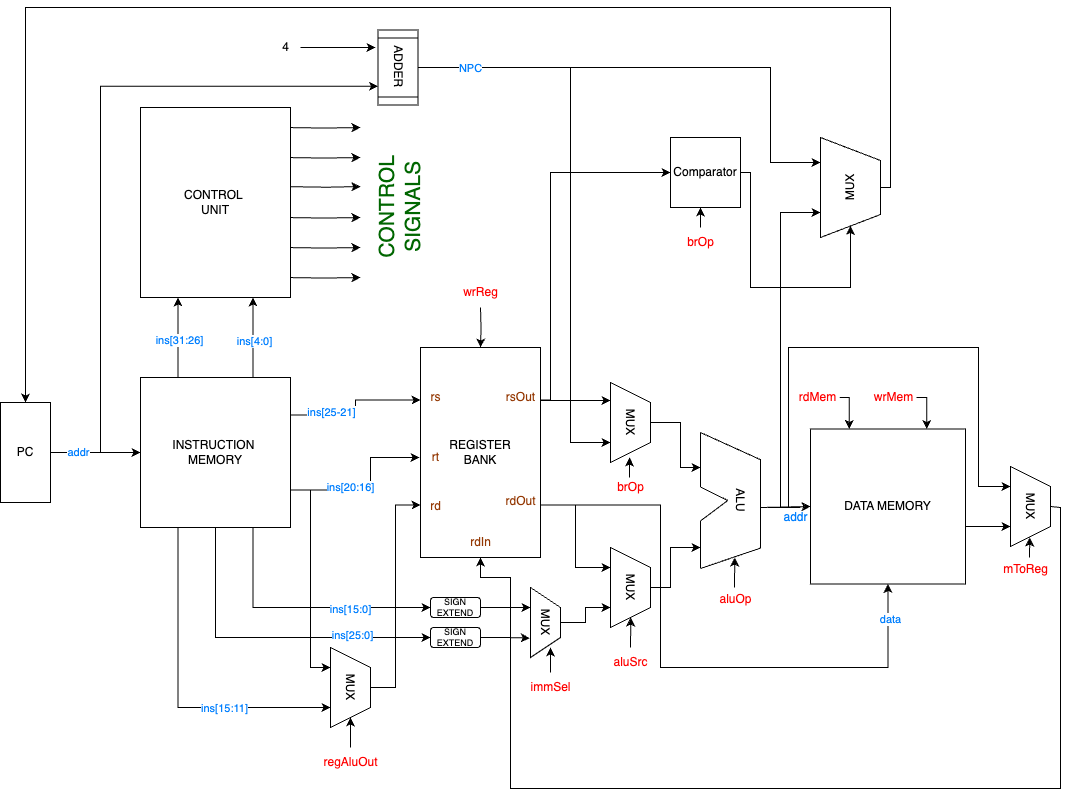
\includegraphics[width=\textwidth]{datapath.png}
    \caption{Processor Datapath}
\end{figure}

\section{Control Unit}

\subsection{aluOp}
\begin{table}[H]
    \centering
    \begin{tabular}{|c|c|c|}
        \hline
        \textbf{Opcode} & \textbf{aluOp} & \textbf{Meaning} \\
        \hline
        000000 & $ins_{3:0}-1$ & Infer from func: ADD,...,HAM \\
        000001-001111 & $ins_{29:26}-1$ & Infer from opcode: ADD,...,HAM \\
        010000 & 1111 & LUI \\
        010001,010010 & 0000 & ADD (for load,store)\\
        010100,010101 & 0000 & ADD (for move) \\
        100000-100011 & 0000 & ADD (for branch) \\
        other & xxxx & Don't Care \\
        \hline
    \end{tabular}
    \caption{Specification of ALU operations}
\end{table}

\subsection{brOp}
\begin{table}[H]
    \centering
    \begin{tabular}{|c|c|c|}
        \hline
        \textbf{Opcode} & \textbf{brOp} & \textbf{Meaning} \\
        \hline
        100000 & 000 & BR \\
        100001 & 001 & BMI \\
        100010 & 010 & BPL \\
        100011 & 011 & BZ \\
        other & 100 & Not a branching instruction \\
        \hline
    \end{tabular}
    \caption{Specification of Branch operations}
\end{table}

\subsection{aluSrc}
\begin{table}[H]
    \centering
    \begin{tabular}{|c|c|c|}
        \hline
        \textbf{Opcode} & \textbf{aluSrc} & \textbf{Meaning} \\
        \hline
        000000 & 1 & rt \\
        other & 0 & imm \\
        \hline
    \end{tabular}
    \caption{Selection of 2nd source of ALU input}
\end{table}

\subsection{regAluOut}
\begin{table}[H]
    \centering
    \begin{tabular}{|c|c|c|}
        \hline
        \textbf{Opcode} & \textbf{regAluOut} & \textbf{Meaning} \\
        \hline
        000000,010100-010101 & 1 & rd \\
        000001-010001 & 0 & rt \\
        other & x & Don't Care \\
        \hline
    \end{tabular}
    \caption{Selection of Destination Register}
\end{table}

\subsection{rdMem}
\begin{table}[H]
    \centering
    \begin{tabular}{|c|c|c|}
        \hline
        \textbf{Opcode} & \textbf{rdMem} & \textbf{Meaning} \\
        \hline
        010001 & 1 & READ from \#imm(R[rs]) \\
        other & 0 & Don't Read \\
        \hline
    \end{tabular}
    \caption{Read from Memory}
\end{table}

\subsection{wrMem}
\begin{table}[H]
    \centering
    \begin{tabular}{|c|c|c|}
        \hline
        \textbf{Opcode} & \textbf{wrMem} & \textbf{Meaning} \\
        \hline
        010010 & 1 & WRITE to \#imm(R[rs]) \\
        other & 0 & Don't Write \\
        \hline
    \end{tabular}
    \caption{Write to Memory}
\end{table}

\subsection{wrReg}
\begin{table}[H]
    \centering
    \begin{tabular}{|c|c|c|}
        \hline
        \textbf{Opcode} & \textbf{wrReg} & \textbf{Meaning} \\
        \hline
        000000-010001,010100-010101 & 1 & Write to dest reg \\
        other & 0 & Don't Write \\
        \hline
    \end{tabular}
    \caption{Write to Register}
\end{table}

\subsection{mToReg}
\begin{table}[H]
    \centering
    \begin{tabular}{|c|c|c|}
        \hline
        \textbf{Opcode} & \textbf{mToReg} & \textbf{Meaning} \\
        \hline
        000000-010000,010100-010101 & 0 & Value from ALUOut \\
        010001 & 1 & Value from LMD \\
        other & x & Don't Care \\
        \hline
    \end{tabular}
    \caption{Source of value to be written to dest reg}
\end{table}

\subsection{immSel}
\begin{table}[H]
    \centering
    \begin{tabular}{|c|c|c|}
        \hline
        \textbf{Opcode} & \textbf{immSel} & \textbf{Meaning} \\
        \hline
        000001-010010,100001-100011 & 0 & $(ins_{15})^{16}\#\#ins_{15:0}$ \\
        100000 & 1 & $ins_{25:0}\#\#00$ \\
        other & x & Don't Care \\
        \hline
    \end{tabular}
    \caption{Selection of sign extended IMM (I-type or J-type)}
\end{table}

\subsection{isCmov}
\begin{table}[H]
    \centering
    \begin{tabular}{|c|c|c|}
        \hline
        \textbf{Opcode} & \textbf{isCmov} & \textbf{Meaning} \\
        \hline
        010101 & 1 & CMOV \\
        other & 0 & not CMOV \\
        \hline
    \end{tabular}
    \caption{Specification of CMOV operation}
\end{table}

\end{document}
